\documentclass[12pt, a4paper]{report}
\NeedsTeXFormat{LaTeX2e}


\newcommand{\YERITHyerithcamerounITEM}[1]
{
\includegraphics[scale=0.03]{images/YERITH-ERP-9-0-CAMEROUN-DRAPEAU.png} #1}


\makeindex

%---------------------------- PACKAGE INCLUSION -------------------------------
% This group renders characters clearer and more precise

\RequirePackage[bitstream-charter,cal,expert]{mathdesign}
\RequirePackage{makeidx}
\RequirePackage{latexsym}

\usepackage[numbib]{tocbibind}


\usepackage{geometry}
\geometry{a4paper,
		  %showframe=true,
		  %margin=2.75em,
		  %a4paper,
		  %total={170mm,257mm},
		  top=4.5em,
		  left=4.5em,
		  right=4.5em,
		  bottom=4em
		  }
		  
%############# COMMAND TO SWITCH SECTION TITLE AND NUMBER COLOR #############
\usepackage{titlesec}

		  
%COMMAND TO MODIFY CELL TABLE ROW HEIGHT
\usepackage{stackengine}
\newcommand\xrowht[2][0]{\addstackgap[.5\dimexpr#2\relax]{\vphantom{#1}}}
		  
		  
\usepackage{multicol}  
		  
\usepackage{alltt}				% support for verbatim text with font specification. e.g: \textbf
\renewcommand{\ttdefault}{txtt}	   % support for verbatim text with font specification. e.g: 		  
		  
	
\newcommand{\SWITCHsectioncolor}[1]{
\titleformat{\section}
{\color{#1}\normalfont\Large\bfseries}
{\color{#1}\thesection}{1em}{}
}		  
		  
		  
\usepackage[default]{cantarell}
\usepackage{graphicx}
\usepackage{xspace}
\usepackage[parfill]{parskip} % Activate to begin paragraphs with an empty line rather than an indent
\usepackage{paralist} % very flexible & customisable lists (eg. enumerate/itemize, etc.)
\usepackage{listings} % for lstset definitions
\usepackage{url}
\usepackage{subfig} % make it possible to include more than one captioned figure/table in a single float
\usepackage{epsfig}
\usepackage{booktabs}
%\usepackage{enumitem} %funny itemize icons
\usepackage{verbatim}
\usepackage{tcolorbox}

\usepackage{pagecolor}

\usepackage{amsmath}
\newcommand{\mathbold}[1]{\text{\textbf{#1}}}



\usepackage{appendix}
\usepackage{tabularx,caption}



\newcommand{\YrtabularxRaggedRIGHTtextsized}[1]
	{#1\raggedleft\arraybackslash}

\newcommand{\YrtabularxRaggedRIGHT}[1]
	{\small\raggedleft\arraybackslash}
	
	
\newcommand{\YrtabularxRaggedLeftTextsized}[1]
	{#1\raggedright\arraybackslash}

\newcommand{\YrtabularxRaggedLeft}[1]
	{\small\raggedright\arraybackslash}
	

\newcommand{\YrtabularxCenteringTEXTSIZE}[1]
	{#1\centering\arraybackslash}

\newcommand{\YrtabularxCentering}[1]
	{\small\centering\arraybackslash}

\newcommand{\numberyr}[1]
	{\scriptsize $#1$.\ \xspace}



\usepackage{xcolor}
\definecolor{yerithColorGOLD}{RGB}{204, 162, 14} 
\definecolor{yerithColorOrange}{RGB}{242, 161, 0}  
\definecolor{yerithColorDarkOrange}{RGB}{198, 70, 00}   
\definecolor{yerithColorYellow}{RGB}{2, 200, 212}   
\definecolor{yerithColorYELLOWrotarian}{RGB}{248, 228, 92}   
\definecolor{yerithColorSILVER}{RGB}{90 , 90 , 90}
\definecolor{yerithColorDarkBlue}{RGB}{77, 95, 180}
\definecolor{yerithColorBlue}{RGB}{77 , 93 , 254}
\definecolor{yerithColorRed}{RGB}{254, 48 , 48}
\definecolor{yerithColorDarkred}{RGB}{165, 29, 45}
\definecolor{yerithColorGray}{RGB}{198, 198, 198}
\definecolor{yerithColorDarkgray}{RGB}{60, 60 , 60}
\definecolor{yerithColorIndigo}{RGB}{83, 0, 125}
\definecolor{yerithColorGreen}{RGB}{2  , 160, 70}
\definecolor{forestgreen}{RGB}{2,160,70}    
\definecolor{mediumblue}{RGB}{7,43,205}    
\definecolor{firebrickred}{RGB}{178,34,34}
\definecolor{listingray}{gray}{0.9}
\definecolor{lbcolor}{rgb}{0.9,0.9,0.9}
\definecolor{yerithColorDarkgreen}{rgb}{0,0.35,0}
\definecolor{medgreen}{rgb}{0,0.5,0}
\definecolor{lightgreen}{rgb}{0.5,0.7,0.5}
\definecolor{pmcolour}{rgb}{0.5,0.7,0.5}
\definecolor{medgrey}{rgb}{0.6,0.6,0.6}
\definecolor{purplish}{rgb}{0.4,0,0.6}
\definecolor{brightred}{rgb}{1,0.2,0.2}

\usepackage{afterpage}

\newcommand\blankpage{%
    \null
    \thispagestyle{empty}%
    \addtocounter{page}{-1}%
    \newpage}



\newcommand{\yrCOLORindigo}[1]
	{\textcolor{yerithColorIndigo}{#1}}
	
	
\newcommand{\yrCOLORDarkblue}[1]
	{\textcolor{yerithColorDarkBlue}{#1}}
	

\newcommand{\yrCOLORDarkorange}[1]
	{\textcolor{yerithColorDarkOrange}{#1}}

\newcommand{\yrCOLORblack}[1]
	{\textcolor{black}{#1}}

\newcommand{\yrCOLORDarkred}[1]
	{\textcolor{yerithColorDarkred}{#1}}
	
	
\newcommand{\yrCOLOR}[2]
	{\textcolor{#1}{#2}}
	
	
\newcommand{\yrCOLORgold}[1]
	{\textcolor{yerithColorGOLD}{#1}}


\newcommand{\yriBigStarGOLDColored}
	{\yrCOLORgold{$\bigstar$}\xspace}



\newcommand{\mytime}[2]{$#1$:$#2$\xspace}


\newcommand{\wy}{WYSIWYG\xspace}

\newcommand{\cplusplus}{\texttt{C}$^{++}$\xspace}

\newcommand{\JAVASCRIPT}{\texttt{JAVASCRIPT}\xspace}

\newcommand{\JAVA}{\texttt{JAVA}\xspace}


\newcommand{\yrilABElCAPTIONofTableWithVSPACEreducingSpaceBELOW}[3]
{
 \captionof{table}{{\footnotesize #3}}
 \label{#2}
 \vspace*{#1}
}


\newcommand{\diplinfn}{DR.\xspace}

\newcommand{\pos}{Progiciel de Gestion Intégré\xspace}

\newcommand{\yerithrd}{\textcolor{yerithColorGOLD}
			{\textsc{\textcolor{yerithColorDarkBlue}{YERITH}}$_{\text{r\&d}}$}\xspace}

\newcommand{\yerithpgi}{YERITH--PGI--$9.0$\xspace}

\newcommand{\yeritherp}{YERITH--ERP--$9.0$\xspace}

\newcommand{\yerithpgicolored}{\textcolor{yerithColorDarkBlue}{\sc YERITH--PGI--$9.0$}\xspace}

\newcommand{\yeritherpcolored}{\textcolor{yerithColorDarkBlue}{\sc YERITH--ERP--$9.0$}\xspace}
	

\newcommand{\PHDxavieryerithnissiHREF}{academic equiv. to a PhD\xspace}


\newcommand{\myfullacademicname}{''\underline{Xavier} Noumbissi \underline{Noundou} [Pr.\ \ Prof.\ \ Dr.--Ing.]'' \xspace}

\usepackage{cite}

\usepackage{etoolbox}


\usepackage[normalem]{ulem} %% \usepackage[normalem]{ulem} \sout{Hello World}  OR \usepackage{soul} \st{Hello World}


\usepackage{hyperref}
\hypersetup{
    colorlinks,
    hyperindex=true,
	pagebackref,
	urlcolor=medgreen,
    citecolor=medgreen,
    linkcolor=purplish,
    breaklinks,
    pdftex,
    bookmarks,
    plainpages=false,
	pdftitle={Configurations-DATA module for \yeritherp; 
				Written by: \myfullacademicname},
    pdfauthor={\myfullacademicname}
}

%--------------------------------------------------------------------------------


% format two pieces of text, one left aligned and one right aligned
\newcommand{\headerrow}[2]
{\begin{tabular*}{\linewidth}{l@{\extracolsep{\fill}}r}
	{\small #1} &
	{\small #2} \\
\end{tabular*}}


\newcommand{\headerrowPARBOXparameter}[2]{\headerrow{\parbox{#1}{#2}}{}}

\newcommand{\headerrowONE}[1]{\headerrow{\parbox{45em}{#1}}{}}


%---------------------------- COMMANDS DEFINITION -------------------------------
\newcommand{\diplinf}{\emph{DR.}\xspace}


\newcommand{\yremphsc}[1]{\textsc{\emph{#1}}\xspace}	

\newcommand{\yremphscBF}[1]{\textsc{\emphbf{#1}}\xspace}


\newcommand{\emphbf}[1]{\emph{\textbf{#1}}\xspace}
\newcommand{\emphit}[1]{\emph{\textit{#1}}\xspace}
\newcommand{\mycheckmark}[1]{\textcolor{#1}{$\checkmark$}\xspace}
\newcommand{\mycheckmarkRESEAU}[1]{{\hfill (\mycheckmark{yerithColorBlue}: #1)}\xspace}
\newcommand{\mycheckmarkACCESSOIRES}[1]{{(\mycheckmark{yerithColorRed}: #1)}\xspace}
\newcommand{\mytimes}[1]{\textcolor{#1}{$\times$}\xspace}
\newcommand{\boldsc}[1]{\textbf{\textsc{#1}}\xspace}

\newcommand{\myenumitem}[1]{\emph{#1}\xspace}


\newcommand{\yrihttpsurl}[1]{\colorlet{links}{yerithColorGreen}\url{https://#1}}

\newcommand{\yrurl}[1]{\colorlet{links}{yerithColorGreen}\url{#1}}

\newcommand{\yrhrefColorORIGINAL}[3][yerithColorDarkgreen]{\href{#2}{\color{#1}{#3}}}

\newcommand{\yrhrefREDColoredNOUNDERLINED}[3][yerithColorDarkred]{\href{#2}{\color{#1}{#3}}}

\newcommand{\yrhrefREDColored}[3][yerithColorDarkred]{\underline{\href{#2}{\color{#1}{#3}}}}

\newcommand{\yrhrefBLACKColored}[3][black]{\href{#2}{\color{#1}{#3}}}

\newcommand{\yrhref}[3][yerithColorDarkgreen]{\href{#2}{\color{#1}{#3}}}


\newcommand{\yrihttps}[3][yerithColorDarkgreen]{\href{https://#2}{\color{#1}{#3}}}


\newcommand{\yrfootnoteurl}[2]{\yremphscBF{#2}~\footnote{\yrurl{#1}}\xspace}

\newcommand{\yrtexturl}[2]{\yremphscBF{#2}~(\yrurl{#1})\xspace}


\newcommand{\yrihttpsfootnoteurl}[2]{\yremphscBF{#2}~\footnote{\yrurl{https://#1}}\xspace}

\newcommand{\yrihttpstexturlSized}[3]{\yremphscBF{#2}~({#3 \yrurl{https://#1}})\xspace}


\newcommand{\yrihttpstexturlONtextToo}[2]{\yremphscBF{\yrihttps{#1}{#2}}~(\yrurl{https://#1})\xspace}


\newcommand{\yrihttpstexturl}[2]{\yremphscBF{#2}~(\yrurl{https://#1})\xspace}


\newcommand{\cscs}{Closed Source Code Software (CSCS)\xspace}

\newcommand{\foss}{Free Open Source Code Software (FOSS)\xspace}

\newcommand{\yerithqvge}{\texttt{YERITH\_QVGE}\xspace}

\newcommand{\yriqvge}{\texttt{YRI\_QVGE}\xspace}


\newcommand{\yrisdmealy}{state diagram mealy machine\xspace}

\newcommand{\yriscriptsized}[1]{{\footnotesize \textsc{#1}}}

\newcommand{\yridbruntimeverif}{\yriscriptsized{YRI-DB-RUNTIME-VERIF}\xspace}
\newcommand{\yrisdruntimeveriflang}{\yriscriptsized{YRI\_SD\_RUNTIME\_VERIF\_LANG}\xspace}
\newcommand{\yrisdruntimeverifUNITTESTS}{\yriscriptsized{YRI\_SD\_RUNTIME\_VERIF\_UNIT\_TESTS}\xspace}
\newcommand{\yrisdruntimeveriflangcomp}{\yriscriptsized{YRI\_SD\_RUNTIME\_VERIF\_LANG\_COMP}\xspace}

\newcommand{\weblinkyrisdruntimeveriflangcomp}
	{\yriurl{https://www.github.com/yerithrd/yri_sd_runtime_verif_lang}\xspace}
	
\newcommand{\weblinkyrisdruntimeverifUNITTESTS}
	{\yriurl{https://www.github.com/yerithrd/yri_sd_runtime_verif_UNIT_TESTS}\xspace}

\newcommand{\weblinkyrisdruntimeveriflang}
	{\yriurl{https://www.github.com/yerithrd/yri_sd_runtime_verif}\xspace}

\newcommand{\weblinkyridbruntimeverif}
	{\yriurl{https://www.github.com/yerithrd/yri-db-runtime-verif}\xspace}



\newcommand{\HREFlinkSPLASHICTSS}[1]
	{\yritexturl{https://zenodo.org/record/8051303}{#1}\xspace}


\newcommand{\HREFlinkJHNISSICOMPENDIUM}[1]
	{\yritexturl{https://zenodo.org/record/8052724}{#1}\xspace}
	
	
\newcommand{\HREFlinkYERITHPGIERPTHREEZERO}[1]{\yrihref{https://www.github.com/yerithrd/yerith-erp-9-0}{#1}\xspace}


\newcommand{\HREFlinkYRQVGE}[1]
	{\yritexturl{https://zenodo.org/record/8387240}{#1}\xspace}

	
\newcommand{\HREFlinkzenodoorgYRQVGE}[1]
	{\yritexturl{https://zenodo.org/records/10070127}{#1}\xspace}

	
\newcommand{\WEBLINKYRQVGEstttattemptjournalarticle}{\yriurl{https://zenodo.org/records/10070127}\xspace}



\newcommand{\yriLabelFORTABLEFigureWITHvspace}[2]{\label{#2}\vspace*{#1}}

\newcommand{\yriLabelFORTABLEFigure}[1]{\label{#1}\vspace*{0.00em}}



\newcommand{\rootcommand}[1]{
\begin{center}
\textcolor{purplish}{#1\xspace}
\end{center}}


\newcommand{\YRFILEEXECUTABLE}{"\textbf{yerith-erp-9-0-standalone-ENGLISH.deb}"\xspace}
\newcommand{\YRFILEconfigurationdata}{"\textbf{yerith-erp-9-0-standalone-configurations-data-ENGLISH.deb}"\xspace}
\newcommand{\YRFILESYSTEMDAEMON}{"\textbf{yerith-erp-9-0-system-daemon.deb}"\xspace}



\newcommand{\AptDebianPACKAGEManagement}{\texttt{apt}\xspace}

\newcommand{\gdebigtk}{\texttt{gdebi-gtk}\xspace}

\newcommand{\gdebi}{\texttt{gdebi}\xspace}

\newcommand{\expect}{\texttt{expect}\xspace}

\newcommand{\debian}{''debian''\xspace}

\newcommand{\debianlinux}{Debian Linux\xspace}

\newcommand{\mswindows}{MS~Windows\xspace}


\newcommand{\qtdbus}{\texttt{Qt-Dbus}\xspace}

\newcommand{\mariadb}{MariaDB\xspace}

\newcommand{\mysql}{MySQL\xspace}

\newcommand{\qt}{Qt$5$\xspace}

\newcommand{\yerithfield}[1]{\textbf{\emph{#1}}\xspace}
\newcommand{\procparagraph}[1]
	{\paragraph{ \mycheckmark{forestgreen} \emph{\textcolor{forestgreen}{#1}}}}


\newcommand{\xavier}{''\underline{Xavier} Noumbissi \underline{Noundou} [Pr.\ \ Prof.\ \ Dr.--Ing.]'' \xspace}


\newcommand{\IMMEUBLEYERITH}{\textcolor{yerithColorDarkBlue}
	{"Immeuble \YERITHyerithcamerounITEM{YERITH"}}\xspace}


\newcommand{\yricellphone}{$(+237)\ 6\ 52\ 39\ 69\ 50$\xspace}


\newcommand{\YERITHCHAPINTRO}[1]{
\begin{center}
\parbox{42em}{
\textcolor{yerithColorIndigo}{#1}
}\xspace
\end{center}}


%--------------------------------------------------------------------------------

\usepackage[T1]{fontenc}
\newcommand{\changefont}[3]{
\fontfamily{#1} \fontseries{#2} \fontshape{#3} \selectfont}
\changefont{cmss}{m}{n}

% Set font to avant-garde
%\renewcommand*\rmdefault{pag}

%%%%%%%%%%%%%%%%%%%%SETTING HEADER AND FOOTER FOR 'REPORT CLASS'.%%%%%%%%%%%%%%%%%%%%%
\usepackage{lastpage}
\usepackage{fancyhdr}
\pagestyle{fancy}
\renewcommand{\headrulewidth}{0pt}
\fancyhf{}

\fancypagestyle{plain}{% copies "fancy" over "plain"
  \fancyfoot[C]{\thepage\ DE \pageref{LastPage}}% you can add edits that won't affect "fancy" but only "plain"
}

\fancypagestyle{OnlyFirstPage}{%
	\lhead{}
	\rhead{}
    \lfoot{}
    \rfoot{}
    \cfoot{\hrule \vspace*{0.03em}
    		\yerithrd -- \IMMEUBLEYERITH -- barrière-Simbock -- Yaoundé VI -- Cameroon}
}


\usepackage{titlesec}
\titleformat*{\subsubsection}{\color{firebrickred}}


\rhead{{\bf \scriptsize Configurations-DATA module for \yeritherp}}
\lhead{\textbf{\yerithrd}}
\lfoot{}
\rfoot{{\footnotesize \today}}
\cfoot{{\footnotesize \thepage\ DE \pageref{LastPage}}}

%Remove widows and orphants
\hyphenpenalty = 10000
\clubpenalty = 10000
\widowpenalty = 10000
\displaywidowpenalty = 10000


\renewcommand\labelenumi{\theenumi)}

\pagenumbering{arabic}

\pdfminorversion=7

\begin{document}

\small

\sloppy

\thispagestyle{OnlyFirstPage}

{} {\bf \Large \yerithrd}
%\\ \line(1,0){450}

\vspace*{1em}

{\hfill \small Version of --~\today~--}

\vspace*{1em}

{
\LARGE 
\begin{center}
\uppercase{
	Booklet on GENERATION of \\
	Configurations-DATA module \\
	for \yeritherp \\
}
\end{center}
}


\vspace*{3em}


\begin{center}
\large
\myfullacademicname
\end{center}

\vspace*{2.5em}

{
\begin{center}
\scriptsize
\yerithrd\\
\IMMEUBLEYERITH \\
barrière-Simbock \\
\vspace*{0.75em}
Yaoundé VI, Cameroon \\
Email: YERITH.xavier@gmail.com
\end{center}
}


\vspace*{3.9em}


\begin{center}
\label{fig:yeritherpcolored-BUSINESS-Workflow}

\includegraphics[scale=0.59]{images/Yerith-erp-pgi-Workflow-BUSINESS.pdf}
\captionof{figure}{\yeritherpcolored~BUSINESS Workflow}
\end{center}



\newpage


\begin{center}
\label{fig:yeritherpcolored-COMPONENTS-Workflow}
\captionof{figure}{\yeritherpcolored~COMPONENTS Workflow}

\includegraphics[scale=0.59]{images/Yerith-erp-pgi-Workflow-Components.pdf}
\end{center}



\cleardoublepage
\blankpage


%%%%%%%%%%%%%%%%%%%%%%%% ABSTRACT %%%%%%%%%%%%%%%%%%%%%%%%%%%%

\newcommand{\libfsmtest}{\texttt{libfsmtest}\xspace}

\newcommand{\tooldejavu}{\texttt{DejaVu}\xspace}

\newcommand{\yrivalgrind}{"\texttt{Valkyrie~/~Valgrind}"\xspace}

\newcommand{\yripurify}{"\texttt{Purify}"\xspace}

\newcommand{\yrilogscope}{"\textsc{LogScope}"\xspace}	


\phantomsection
\addcontentsline{toc}{chapter}{Abstract}
\begin{abstract}
\thispagestyle{OnlyFirstPage}
\begin{center}

\vspace*{0.49em}

\parbox{41.00em}{
	
{ \small
\yremphscBF{THIS document explains mainly 
how to generate configurations data for 
Enterprise Resource Planing (ERP;~\textcolor{yerithColorGOLD}{[PGI in French language]})
software \yeritherp; from the command line, 
on a \debianlinux programming environment.}
}
}
\end{center}
\end{abstract}


%%%%%%%%%%%%%%%%%%%%%%%% TABLE DES MATIÈRES %%%%%%%%%%%%%%%%%%%%%%%%%%%%

\cleardoublepage
\blankpage


% TABLE OF CONTENTS
\phantomsection
%\addcontentsline{toc}{chapter}{\contentsname}
\begingroup
\tableofcontents
\endgroup


\cleardoublepage
\blankpage


% LIST OF FIGURES
\phantomsection
%\addcontentsline{toc}{chapter}{\listfigurename}
\begingroup
\color{medgreen}
\listoffigures
\endgroup


\cleardoublepage
\blankpage


% LIST OF TABLES
\phantomsection
%\addcontentsline{toc}{chapter}{\listtablename}
\begingroup
\color{medgreen}
\listoftables
\endgroup


\cleardoublepage
\blankpage


\chapter{Introduction}

\YERITHCHAPINTRO{
	\yremphsc{This chapter shows how to generate the
	debian package named 'yerith-erp-9-0-standalone-configurations-data-ENGLISH.deb'
	(\yrCOLORgold{or 'yerith-erp-9-0-standalone-configurations-data.deb'
	as FRENCH-language version}) for configuring the 
	ERP software \yeritherp.}
}



\vspace*{0.95em}



\section{Prerequisite Software}

%\vspace*{1em}

\begin{table}[!htbp]
\centering
\captionof{table}{Prerequisite software.}
\label{tab:prerequisite-software}
\begin{tabularx}{\textwidth}{X|X}
\hspace*{.2\textwidth} \textbf{Software}	&
\hspace*{.2\textwidth} \textbf{Versions}	\\ \hline
\end{tabularx}
\begin{tabularx}{\textwidth}{>{\small}X | >{\small\hfill\arraybackslash}X}
\gdebi				&
$0.9.5.7+nmu5$		\\
\end{tabularx}
\end{table}



\vspace*{0.95em}



\begin{table}[!htbp]
\centering
\captionof{table}{Files required for installation of \yeritherp.}
\yriLabelFORTABLEFigureWITHvspace{-0.79em}{tab:prerequisite-files}
\begin{tabularx}{\textwidth}{|X|} 						\hline \xrowht{1em}
\hspace*{.47\textwidth} \textbf{\uppercase{Files}}		\\ \hline \xrowht{0.72em}
\YRFILEEXECUTABLE											\\ \hline \xrowht{0.72em}
\YRFILEconfigurationdata									\\ \hline \xrowht{0.72em}
\YRFILESYSTEMDAEMON										\\ \hline	
\end{tabularx}
\end{table}

\vspace*{1em}

Table~\ref{tab:prerequisite-files} illustrates files required
for installing \yeritherp.


\vspace*{0.95em}



\section{A Package management file For \debianlinux}

A software system and~/~or module could be installed easily
for the \yrihttpstexturl{www.debian.org}{\debianlinux platform} 
when its is packaged~(archived) as file type 
'.deb'~(or debian package).

\qquad
Such a '.deb'-file contains files and binary executable
and~/~or instructions on how to place them onto the file
system of the computer where to install this software system,
and~/~or program.



\newpage



\section{\yrCOLORDarkred{How to Download \yeritherp sample FOSS source code}}

\begin{enumerate}[$1.)$]
	\itemsep 0.42em
	
	\item From the website \yrihttpstexturl{www.github.com}{''www.github.com''}~:
	
	\qquad
	From your bash shell command, type the following command~:
		\vspace*{-0.15em}	
		\begin{alltt}
			\rootcommand{git clone https://www.github.com/yerithrd/yerith-erp-9-0}
		\end{alltt}			
\end{enumerate}



\section{Set a BASH-path for \yeritherp commands}

\begin{enumerate}[$1.)$]
	
	\itemsep 0.21em

	\item \yremphsc{Open a ''bash--terminal''}
	
	\item \yremphsc{type following lines of Bash-shell code in 
		your '/home/\$USER/.bashrc file'~:}
		
		\vspace*{-0.15em}	

		\begin{verbatim}
			export LD_LIBRARY_PATH=/usr/lib/x86_64-linux-gnu
			export GIT_EDITOR=vim
			QT_SELECT=5
			YERITH_ERP_3_0_HOME_FOLDER=${HOME}/yerith-erp-9-0
			YERITH_ERP_3_0_PROPERTIES_CONFIGURATION_FOLDER=${YERITH_ERP_3_0_HOME_FOLDER}
			YERITH_ERP_3_0_SYSTEM_DAEMON_HOME_FOLDER=$HOME/yerith-erp-9-0-system-daemon
			PATH=${YERITH_ERP_3_0_HOME_FOLDER}/yerith-erp-9-0-development-scripts:${PATH}
			PATH=${YERITH_ERP_3_0_HOME_FOLDER}/yerith-erp-9-0-development-scripts/ENGLISH:${PATH}
			
			export YERITH_ERP_3_0_PROPERTIES_CONFIGURATION_FOLDER

			export YERITH_ERP_3_0_HOME_FOLDER
			
			export YERITH_ERP_3_0_SYSTEM_DAEMON_HOME_FOLDER			
			
			export PATH
			
		\end{verbatim}		
		
		\vspace*{-0.27em}		
		
		\yrCOLORDarkred{\yremphscBF{PLEASE, revert the BASH--settings 
		afore given when re--installing your productive version of 
		\yeritherp so to avoid collisions of BASH environment variables
		specifications~!}}

		
\end{enumerate}



\section{\yrCOLORDarkred{How to generate 'yerith-erp-9-0-standalone-configurations-data-ENGLISH.deb'}}
 
\begin{enumerate}[$1.)$]
	
	\itemsep 0.21em

	\item \yremphsc{Open a ''bash--terminal''}
	
	\item \yremphsc{type following command~:}
		\vspace*{-0.15em}	
		\begin{alltt}
			\rootcommand{yerith-create-dpkg_yerith-erp-9-0-standalone-configurations-data-ENGLISH.sh}
		\end{alltt}
\end{enumerate}



\section{\yrCOLORDarkred{How to generate 'yerith-erp-9-0-standalone-configurations-data.deb'}}
 
\begin{enumerate}[$1.)$]
	
	\itemsep 0.21em

	\item Open a ''bash--terminal''
	
	\item \yremphsc{type following command~:}
		\vspace*{-0.15em}	
		\begin{alltt}
			\rootcommand{yerith-create-dpkg_yerith-erp-9-0-standalone-configurations-data.sh}
		\end{alltt}
\end{enumerate}






\cleardoublepage
\blankpage


\chapter{Installation of a '.deb' File}

\YERITHCHAPINTRO{
	\yremphsc{This chapter shows how to
	Install a \debian package management file.}
}


\vspace*{1.05em}


\begin{center}
\captionof{figure}{Gdebi-gtk user graphical interface.}
\yriLabelFORTABLEFigureWITHvspace{-0.49em}{fig:gdebi-gtk-user-graphical-interface}
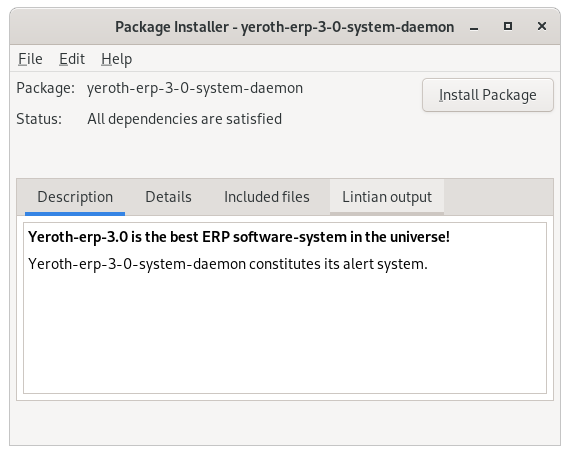
\includegraphics[scale=0.60]{images/YR_GDEBI-GTK.png}
\end{center}


\vspace*{0.95em}


\section{Automated Installation with \gdebigtk and \gdebi}

Program \gdebi and its Graphical User Interface~(GUI)
version \gdebigtk enables one to install a 'deb' file 
without any troubles and~/~or configuration of a \debian 
software packages repository (as for instance in 
file \texttt{''/etc/apt/source.list''}).

\qquad
\yrCOLORDarkred{\gdebi and \gdebigtk have following 
advantage~:~BOTH programs will search all required 
dependent packages--programs and will install them 
automatically for you.}

\qquad
\yrCOLORDarkred{THUS, in this occasion you need to 
configure your \debian software packages repository 
file located at \texttt{''/etc/apt/source.list''}.}



\section{Installation of \gdebigtk and~/~or \gdebi}

\begin{enumerate}[$1.)$]
	\itemsep 0.21em

	\item \yremphsc{Open a ''bash--terminal''}
	
	\item \yremphsc{type following command to install \gdebigtk~:}
		\begin{alltt}
			\rootcommand{apt -y install gdebi-gtk}
		\end{alltt}	
	
	\item \yremphsc{type following command to install \gdebi~:}
		\begin{alltt}
			\rootcommand{apt -y install gdebi}
		\end{alltt}
\end{enumerate} 



\section{Installation with \gdebi}

\begin{enumerate}[$1.)$]
	\itemsep 0.21em

	\item \yremphsc{Open a ''bash--terminal''}
	
	\item \yremphsc{type following command~:}
		\begin{alltt}
			\rootcommand{gdebi -n yerith-erp-9-0-standalone-ENGLISH.deb}
		\end{alltt}
\end{enumerate} 



\section{Installation with \gdebigtk}

\begin{enumerate}[$1.)$]
	\itemsep 0.21em
	
	\item \yremphsc{Open a ''bash--terminal''}
	
	\item \yremphsc{type following command~:}
		\begin{alltt}
			\rootcommand{gdebi-gtk yerith-erp-9-0-standalone-ENGLISH.deb}
		\end{alltt}
		
	\item \yremphsc{press button "Install Package".}
\end{enumerate} 



\newpage




\section{\yremphscBF{\yrCOLORDarkorange{Installation of a Debian Software Repository locally on your Computer}}}

\begin{enumerate}[$1.)$]
	\itemsep 0.21em

	\item 
\end{enumerate} 




\section{\yremphscBF{\yrCOLORDarkred{Installation with \AptDebianPACKAGEManagement Tool}}}

\begin{enumerate}[$1.)$]
	\itemsep 0.21em

	\item \yremphscBF{\yrCOLORDarkorange{Prerequisite~:~You could 
		add all '.deb' into a software \debian repository online.}}
	
	\item \yremphsc{Open a ''bash--terminal''}
	
	\item \yremphsc{type following command~:}
		\begin{alltt}
			\rootcommand{apt -y install yerith-erp-9-0-standalone-configurations-data-ENGLISH}
		\end{alltt}
		
	\item \yremphsc{type following command~:}
		\begin{alltt}
			\rootcommand{apt -y install yerith-erp-9-0-standalone-ENGLISH}
		\end{alltt}

	\item[$\circ$] \yremphscBF{\yrCOLORDarkorange{Or alternatively to the 
		$2$ previous commands, you could issue the following command~:~}}
		{ \scriptsize
		\begin{alltt}
			\rootcommand{apt -y install yerith-erp-9-0-standalone-configurations-data-ENGLISH yerith-erp-9-0-standalone-ENGLISH}
		\end{alltt}
		}
\end{enumerate} 







\cleardoublepage
\blankpage




\newcommand{\yerithpgisystemdaemon}{YERITH--PGI--$9.0$--SYSTEM--DAEMON\xspace}

\newcommand{\elementgraphique}[1]{"\texttt{#1}"\xspace}

\newcommand{\manager}{\emph{Manager}\xspace}
\newcommand{\gestionairedestocks}{\emph{GestionaireDeStocks}\xspace}
\newcommand{\magasinier}{\emph{Magasinier}\xspace}
\newcommand{\caissier}{\emph{Caissier}\xspace}
\newcommand{\vendeur}{\emph{Vendeur}\xspace}
\newcommand{\administrateur}{\emph{Administrateur}\xspace}

\newcommand{\managerb}{\emph{\textbf{Manager}}\xspace}
\newcommand{\gestionairedestocksb}{\emph{\textbf{GestionaireDeStocks}}\xspace}
\newcommand{\vendeurb}{\emph{\textbf{Vendeur}}\xspace}
\newcommand{\caissierb}{\emph{\textbf{Caissier}}\xspace}
\newcommand{\administrateurb}{\emph{\textbf{Administrateur}}\xspace}


\chapter{\yrCOLORgold{Brief Overview of Configuration Data for \yeritherp}}

\YERITHCHAPINTRO{
	\yremphsc{This chapter shows a structure view of how
	configuration data for \yeritherp are organized.}
}


\vspace*{1.05em}


\begin{center}
\captionof{figure}{\yremphscBF{Screenshot of configuration data in administrative section of \yeritherp.}}
\yriLabelFORTABLEFigureWITHvspace{0.00em}{fig:gdebi-gtk-user-graphical-interface}
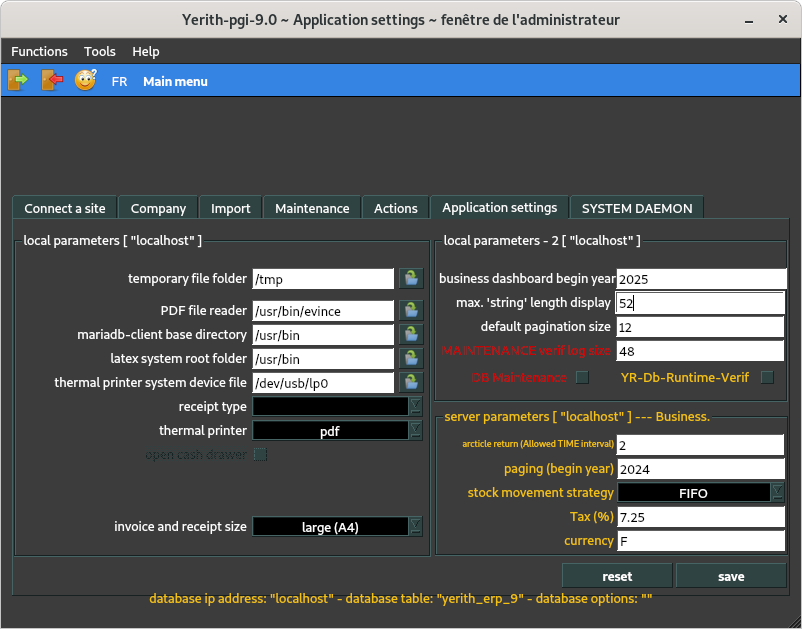
\includegraphics[scale=0.60]{images/Yerith-Erp-Pgi-9-0-Screenshot-configurations-data-Administrative-section.png}
\end{center}


\vspace*{0.95em}



\section{INTRODUCTION}
\index{paramètres locaux}
\index{paramètres serveurs}

\vspace*{1em}

\begin{table*}[!htbp]
\centering
\captionof{table}{Types de paramètres de l'application PGI yeritherp et 
	du système d’alertes et de sauvegardes automatisées.}
\label{tab:parametres-de-lapplication-pgi}
%\resizebox{\textwidth}{!}{%to fit the table within the text width
\begin{tabular}{|c|c|} \hline

\textbf{TYPES DE PARAMÈTRES} 	& 
\textbf{UTILISATEURS MODIFICATEURS}			\\ \hline

paramètres locaux					&
\administrateur, \manager			\\ \hline
		
paramètres serveurs					&
\manager							\\ \hline		

\end{tabular}
%}
\end{table*}

\vspace*{1em}

Tous les paramètres du PGI yeritherp sont
centralisés dans la section \elementgraphique{ADMINISTRATION}.	

Il existe des \textbf{paramètres locaux}
(enregistrés sur le disque dur de l'ordinateur
de l’utilisateur), et des \textbf{paramètres serveurs}
(enregistrés dans la base de données du PGI
yeritherp):

\begin{enumerate}[1.]
	\item Des \textbf{paramètres locaux} influencent
		uniquement des instances du PGI 
		yeritherp dans l'ordinateur de
		l’utilisateur, et sont modifiables par 
		$1$ \administrateurb ou $1$ \managerb.
		
	\item Des \textbf{paramètres serveurs} influencent
		TOUTES LES INSTANCES DU PGI yeritherp
		QUI SONT RATTACHÉES AU SERVEUR DE BASE
		DE DONNÉES EN QUESTION !
		
		Des paramètres serveurs sont modifiables
		UNIQUEMENT par $1$ \managerb.
\end{enumerate}

Tous les types de paramètres et les utilisateurs
responsables de leurs modifications sont illustrés
dans le TABLEAU~\ref{tab:parametres-de-lapplication-pgi}.\\


TOUS PARAMÈTRE LOCAL OU SERVEUR EST SOIT:
\begin{enumerate}[1.]
	\item \emphbf{$1$ paramètre de l'application erp (pgi)}
			(SECTION~\ref{subsec:parametres-de-lapplication-erp-pgi})
	\item \emphbf{$1$ paramètre du système d’alertes et
		de sauvegardes automatisées}
		(SECTION~\ref{subsec:parametres-du-systeme-dalerte-et-de-sauvegarde-automatisee}).
\end{enumerate}


\newpage


\section{PARAMÈTRES DE L'APPLICATION ERP (PGI)}
\index{paramètres de l’application erp (pgi) yeritherp}
\label{subsec:parametres-de-lapplication-erp-pgi}

\vspace*{1em}

\begin{center}
\captionof{figure}{La fen\^etre de paramétrage du PGI yeritherp.}
\label{fig:fenetre-de-visualisation-du-PGI-yerith-erp-9-0}
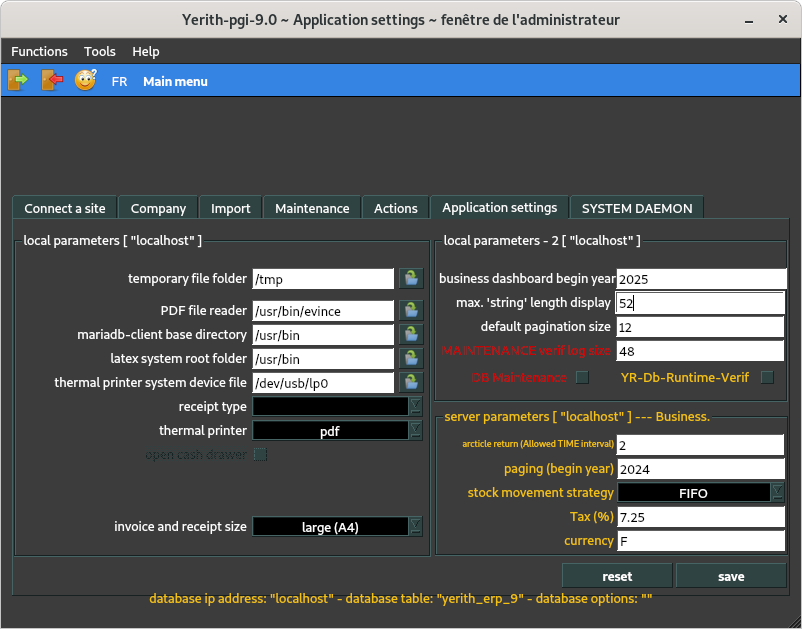
\includegraphics[scale=0.5]{images/Yerith-Erp-Pgi-9-0-Screenshot-configurations-data-Administrative-section.png}
\end{center}

\vspace*{1em}

$1$ paramètre de l’application erp (pgi) yeritherp
est $1$ valeur qui influence ses comportements
du PGI yeritherp lors de son exécution:
\emphbf{le format des reçus ("\emphbf{petit}",
"\emphbf{A$4$}", ou "\emphbf{A$5$}") en est $1$ exemple !}




\subsection{LOCAL parameters --- Computer LOCAL specific}



\subsection{\yrCOLORDarkorange{Server parameters --- BUSINESS--only correlated information}}




\newpage


\section{PARAMÈTRES DU SYSTÈME D'ALERTES ET DE SAUVEGARDE AUTOMATISÉE DE LA
			BASE DE DONNÉES}
\index{paramètres du système d'alertes, et du
	système de sauvegarde automatisée \yerithpgisystemdaemon}
\label{subsec:parametres-du-systeme-dalerte-et-de-sauvegarde-automatisee}

\vspace*{1em}

\begin{center}
\captionof{figure}{La fen\^etre de paramétrage du système d'alertes,
			et du système de sauvegarde automatisée.}
\label{fig:fenetre-de-visualisation-du-systeme-dalerte}
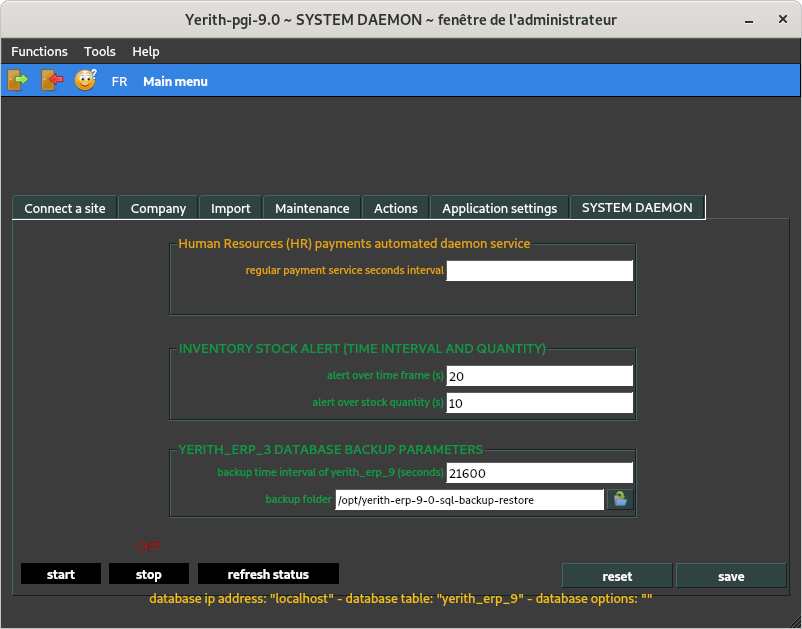
\includegraphics[scale=0.5]{images/yerith-erp-9-0-system-daemon-parameters.png}
\end{center}

\vspace*{1em}

$1$ paramètre du système d'alertes, et du système
de sauvegarde automatisée \yerithpgisystemdaemon est
$1$ valeur qui influence ses comportements lors
de son exécution: \emphbf{le répertoire de sauvegarde des
bases de données \mysql de yeritherp EN EST $1$ EXEMPLE !} 







\cleardoublepage
\blankpage


\chapter{CONCLUSION}

\YERITHCHAPINTRO{
	\yremphsc{This chapter concludes our brief presentation
	on generating \debian package management files for
	\yeritherp; for a \yrihttpstexturl{www.debian.org}{\debianlinux}
	installation environment system.}
}



\vspace*{0.95em}





\end{document}
